
%==============  N E W  ==== C H A P T E R ==============%
\chapter{Vergleich der Ergebnisse}
\label{chapter:Vergleich}

Wie in der Aufgabenstellung (siehe Kapitel \ref{subsec:Ausgangslage}) erw�hnt, sollen die Suchresultate von Lucene mit denjenigen des Betriebssystems verglichen werden. Die Suche im Betriebssystem ist sehr intuitiv. Es wird der gew�nschte Suchbegriff eingegeben und nach ein paar Sekunden (oder Minuten), je nach dem ob alle Ordner indiziert waren oder nicht, erscheint das Resultat.

Die Qualit�t der Suche wird nicht anhand der Geschwindigkeit ermittelt. Anhand der im Kapitel \ref{subsec:eigesetzteHardware} aufgelisteten Hardware w�re es kein fairer Vergleich, eine SSD mit einer herk�mmlichen HDD zu vergleichen.

Um einen Vergleich zu starten, wird ein beliebiges File ausgew�hlt. Danach wird anhand nicht nur diesem File zugeordneten Kriterien gesucht. Eine erlaube Suchanfrage ist zum Beispiel: File enth�lt \flqq beispiel\frqq, eine nicht erlaube Suchanfrage: Der Filename ist \flqq beispiel.txt\frqq.

%==============  N E W  ==== S E C T I O N ==============%
\newpage
\index{Windows 8.1|see{Vergleich mit Windows}}
\index{Vergleich mit Windows|(}
\section{Vergleich Lucene mit Windows 8.1 Pro}
\label{sec:Vergleich Lucene mit Windows 8.1 Pro}

Dei gew�hlte Datei, welche durch die Suche gefunden werden sollte ist: \flqq../1. Jahr/Software Projekt 1/Dokumentation SW Projekt 2. Semester V0.1.docx\frqq

\textbf{Annahme f�r die Suche}
\begin{itemize}
\item Filename ist unbekannt
\item Autor: entweder \flqq micha\frqq\ oder \flqq reto\frqq
\item File Extension: *.doc oder *.docx
\item Im Inhalt muss vorkommen: \flqq Address.java\frqq.
\end{itemize}

%==============  N E W  ==== S U B S E C T I O N ==============%
\subsection{Suche \#1 mit Windows 8.1 Professional}
\label{Suche1 mit Windows 8.1 Professional}

Bei der klassischen Suche im Windows werden die gesuchten Attribute in die Suchmaske eingegeben:
\begin{figure}[h!]
\centering
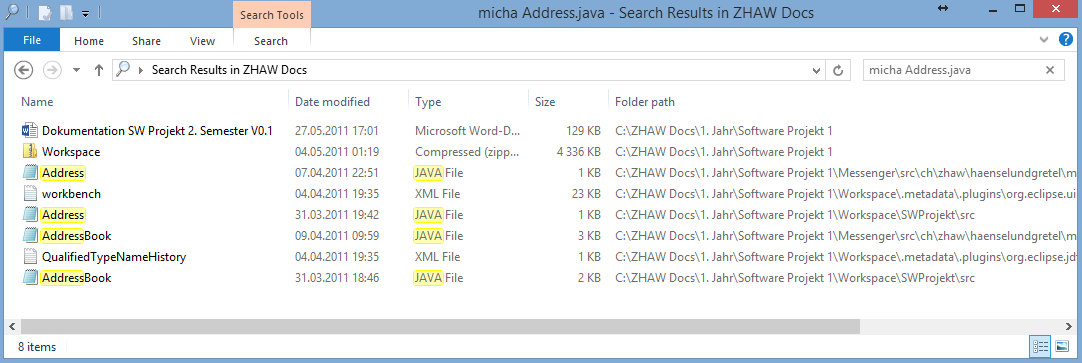
\includegraphics[width=1\textwidth]{Win8_Search1_normal.PNG} 
\caption[Gewohnte Windows Suche 1]{Gewohnte Windows Suche 1\\Quelle: eigener Screenshot}
\label{fig:Gewohnte Windows Suche 1}
\end{figure}
Die meisten Windows-Benutzer w�rden hier 2 Suchanfragen starten. Die erste mit der Suchanfrage \flqq micha Address.java\frqq, die zweite mit \flqq reto Address.java\frqq

Durch das Auseinandersetzen mit der effizienten Windows-Suche wurde klar, dass Windows von Haus aus weit mehr beherrscht als nur nach Stichworten zu suchen. Erweiterte Tipps f�r die Suche mit Windows gibt es von Mircosoft �ber \url{http://windows.microsoft.com/de-ch/windows7/advanced-tips-for-searching-in-windows}.

Werden die fortgeschrittenen Syntax bei der Suche eingehalten, sieht diese Anfrage folgedermassen aus: \flqq authors:~=\grqq micha\grqq\ OR authors:~=\grqq reto\grqq\ AND Address.java\frqq. Diese Anfrage bedeutet, dass entweder \flqq micha\frqq\ oder \flqq reto\frqq\ im Feld Author vorhanden sein muss. Da \flqq Address.java\frqq\ nicht zugeordnet wurde, muss es irgendwo vorkommen.
\begin{figure}[h!]
\centering
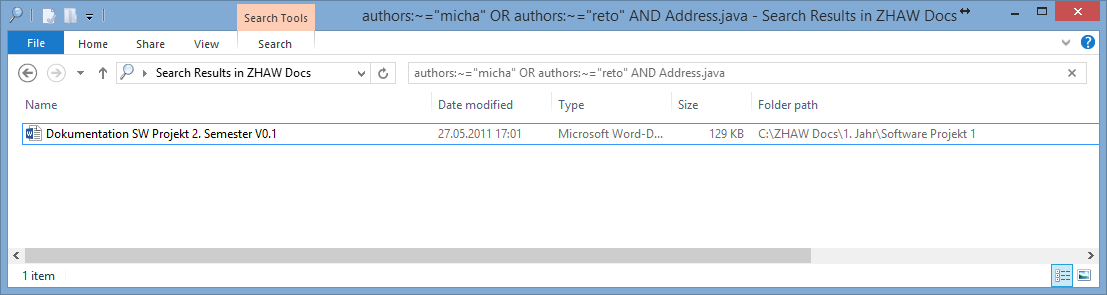
\includegraphics[width=1\textwidth]{Win8_Search1_extended.PNG} 
\caption[Erweiterte Suche 1 mit Windows]{Erweiterte Suche 1 mit Windows\\Quelle: eigener Screenshot}
\label{fig:Erweiterte Suche 1 mit Windows}
\end{figure}
 
Durch den Einsatz des optimierten Syntax f�r die Windows suche l�sst das Resultat mit genau einem File dem Herausforderer Lucene bereits im Vorfeld keine grosse Chance.

%==============  N E W  ==== S U B S E C T I O N ==============%
\subsection{Suche \#1 mit Lucene und Luke}

Die Suche mit Luke, welche auf die von Lucene indizierte Files zugreift, dauerte im Schnitt 300-500$\mu$s.\\
Wie die Abbildung \ref{fig:Suche 1 mit Lucene} zeigt, werden hier mehrere Dateien gefunden. Die gesuchte Datei ist ebenfalls vorhanden (\#11).


\begin{figure}[h!]
\centering
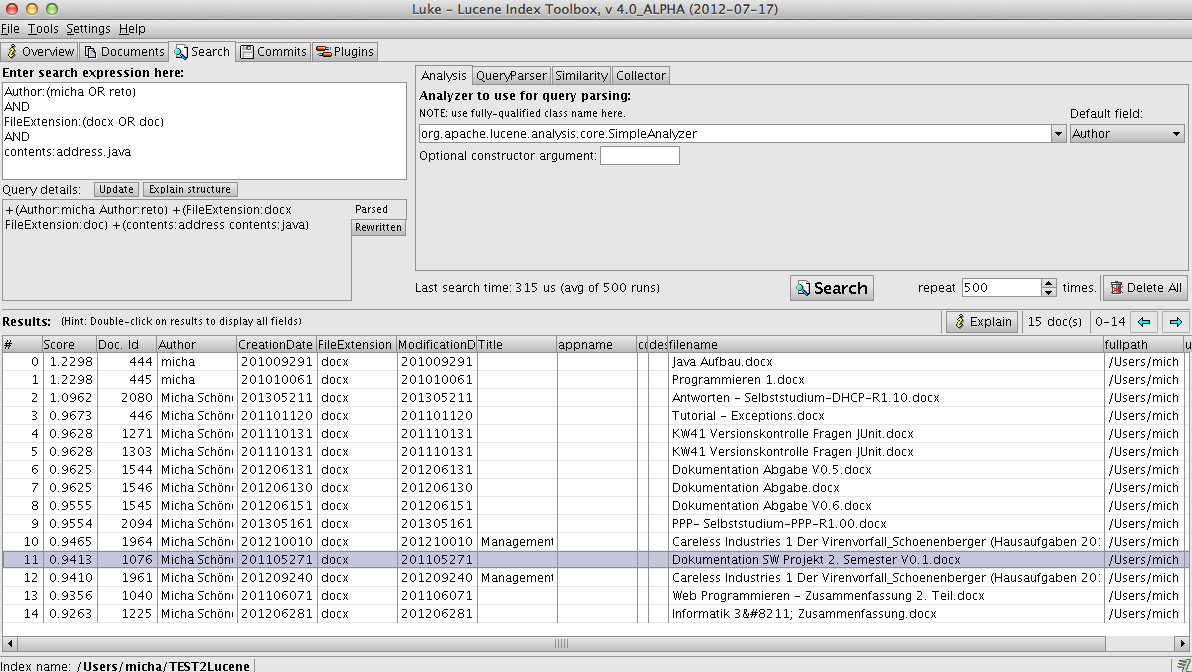
\includegraphics[width=1\textwidth]{Lucene_Search_1.PNG} 
\caption[Suche 1 mit Lucene]{Suche 1 mit Lucene\\Quelle: eigener Screenshot}
\label{fig:Suche 1 mit Lucene}
\end{figure}

%==============  N E W  ==== S U B S E C T I O N ==============%
\subsection{Fazit zur Suche \#1}
\index{Fazit Suchergebnis|(}
Die Windows Search Engine sowie die eigene Lucene Applikation finden beide das gew�nschte Dokument. Beim Windows ist es das einzige Dokument, welches gelistet wird. Lucene hingegen listet das gesuchte Dokument an der 11. Stelle. Ist nun Lucene schlechter deswegen?
Um auf diese Frage eine Antwort zu finden, m�ssen die anderen von Lucene ausgegebenen Dokumenten �berpr�ft werden. Es k�nnte auch sein, dass Lucene alle Dokumente auflistet, Windows jedoch nur per \grqq Zufall\grqq\ das Richtige. Was w�re, wenn das File \grqq Java Aufbau.docx\grqq, welches bei Lucene zuoberst steht, gesucht worden w�re?

Die beiden ersten Dokumente wurden untersucht. Das Fazit hierbei ist, dass alle gesuchten Merkmale bei den Dokumenten vorhanden waren, ausser dem contents:address.java. \flqq address.java\frqq\ wurde in beiden Dokumenten nicht gefunden. Wo liegt der Fehler?


Wird die identische Suche mit Luke nochmals durchgef�hrt, jedoch anstelle des Simple-Analyzer der Standard, German- oder English-Analyzer eingesetzt, findet Lucene genau eine einzige Datei (siehe Abbildung \ref{fig:Suche 1 mit Lucene English Analyzer}). Das Resultat entspricht derjenigen Datei, die gefunden werden sollte.

\begin{figure}[h!]
\centering
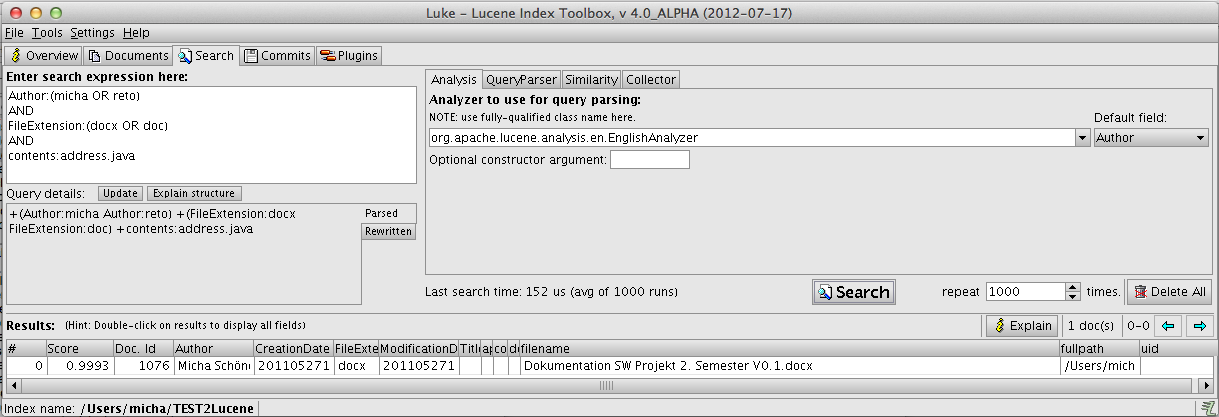
\includegraphics[width=1\textwidth]{Lucene_Search_1_english.PNG} 
\caption[Suche 1 mit Lucene mit English-Analyzer]{Suche 1 mit Lucene mit English-Analyzer\\Quelle: eigener Screenshot}
\label{fig:Suche 1 mit Lucene English Analyzer}
\end{figure}
\index{Fazit Suchergebnis|)}

%==============  N E W  ==== S U B S E C T I O N ==============%
\subsection{Kurzer Exkurs zu Analyzern}
\index{Analyzer|(}
Werden die verschiedenen Analyzer genauer betrachtet, wird das vermeintlich falsche Resultat logisch erkl�rbar.\\
Beim ersten Durchgang mit dem \flqq SimpleAnalyzer\frqq\ wird der indizierte Text bei Nicht-Schriftzeichen (z.B. \flqq .\frqq, \flqq \ \frqq, \flqq !\frqq) getrennt und alle Buchstaben klein geschrieben.\\
Wird nun wie bei der Suche \#1 jedoch \flqq address.java\frqq\ gesucht, �ndert dies der Analyzer zu \flqq address\frqq\ und \flqq java\frqq. Aus diesem Grund sind nun Dokumente auffindbar, welche \flqq address.java\frqq\ nicht enthalten. Bei genaueren Hinschauen sind jedoch die beiden W�rter einzeln vorhanden.

Beim zweiten Durchgang findet Luke genau das gesuchte Dokument. Als Beispiel wird hier der \flqq StandardAnalyzer\frqq\ betrachtet. Dieser basiert auf einer ausgefeilten Grammatik, welche unter anderem alphanumerische, chinesische, japanische oder koreanische Zeichen, E-Mail Adressen, Akronyme und vieles mehr erkennt. Zus�tzlich werden alle Buchstaben wie beim SimpleAnalyzer klein geschrieben. Der  \flqq StandardAnalyzer\frqq\ entfernt ebenfalls Stop-W�rter (auf die hier nicht eingegangen wird).

Anbei ein Auszug aus Luke, bei welchem der Index der gesuchten Datei rekonstruiert wurde. Hier ist ersichtlich, dass \flqq address.java\frqq\ in Zeile 2 korrekt indiziert wurde. Der SimpleAnalyzer erkennt diese beiden W�rter jedoch als zwei W�rter im Gegensatz zum StandardAnalyzer.

\lstset{language=java, mathescape=true}
\lstinputlisting[label=Auszug aus Index von Dokumentation SW Projekt 2. Semester,captionpos=b, caption=Auszug aus Index von Dokumentation SW Projekt 2. Semester]{dir/listings/Suche1.java}

Quelle: \cite{LiA-2ndEdition}, S. 127
\index{Analyzer|)}
\index{Vergleich mit Windows|)}


%==============  N E W  ==== S E C T I O N ==============%
\newpage
\section{Vergleich 2 Lucene mit Windows 8.1 Pro}
\label{sec:Vergleich 2 Lucene mit Windows 8.1 Pro}

Dei gew�hlte Datei, welche durch die Suche gefunden werden sollte ist: \flqq../3. Jahr/Kryptologie/KK 05/05 - Slides der Woche 5.pdf\frqq

\textbf{Annahme f�r die Suche}
\begin{itemize}
\item Filename ist unbekannt
\item Im Inhalt muss vorkommen: \flqq Inverse\frqq
\item File Extension: *.pdf
\end{itemize}




%==============  N E W  ==== S U B S E C T I O N ==============%
\subsection{Suche \#1 mit Windows 8.1 Professional}
\label{Suche1 mit Windows 8.1 Professional}

Zu Beginn soll Windows anhand der klassischen Benutzersuche die Anfrage starten.
\begin{figure}[h!]
\centering
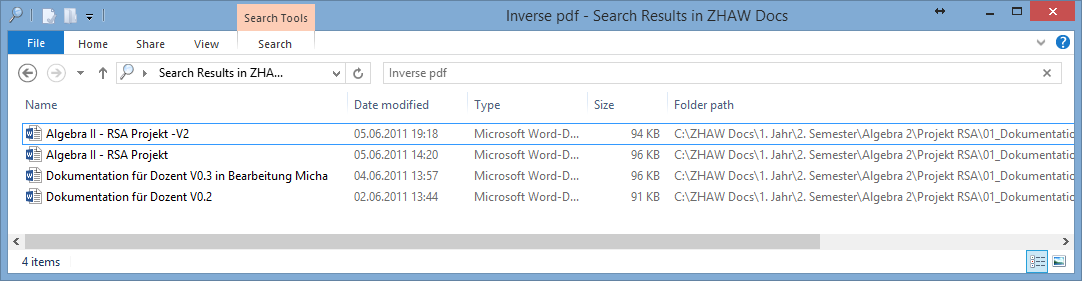
\includegraphics[width=1\textwidth]{Win8_Search2_normal.PNG} 
\caption[Gewohnte Windows Suche 2]{Gewohnte Windows Suche 2\\Quelle: eigener Screenshot}
\label{fig:Gewohnte Windows Suche 2}
\end{figure}

 Die Abbildung \ref{fig:Gewohnte Windows Suche 2} zeigt, dass das gew�nschte Dokument nicht vorhanden ist.\\
 Deshalb wird nun versucht, mit dem erweiterten Windows Syntax das Dokument zu suchen:
 
\begin{figure}[h!]
\centering
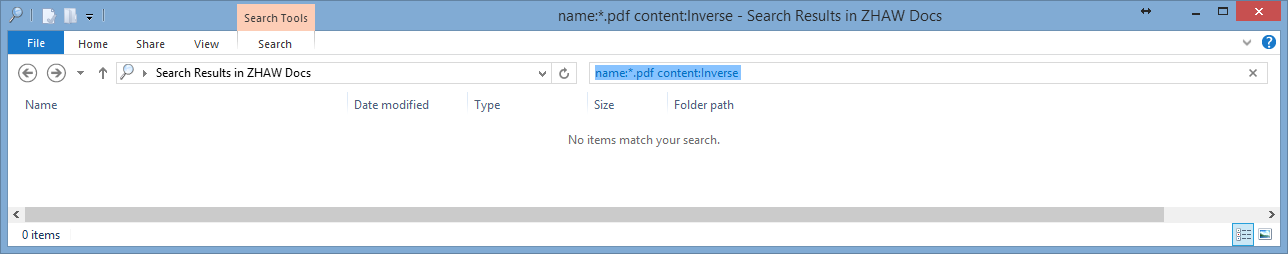
\includegraphics[width=1\textwidth]{Win8_Search2_extended_1.PNG} 
\caption[Erweiterte Suche 2 mit Windows 1]{Erweiterte Suche 2 mit Windows 1\\Quelle: eigener Screenshot}
\label{fig:Erweiterte Suche 2 mit Windows1}
\end{figure}
 
 Wie nicht anders erwartet, liefert Windows keine richtige Antwort, wie Abbildung \ref{fig:Erweiterte Suche 2 mit Windows1} zeigt. Da bereits die herk�mmliche Suche, welche nur nach \flqq Invers\frqq\ und \flqq pdf\frqq\ gesucht hat, kein einziges PDF gefunden hat, ist es nicht verwunderlich, dass bei der erweiterten Suche keine Treffer gab.
 
Untenstehende Abbildung \ref{fig:Erweiterte Suche 2 mit Windows2} zeigt jedoch, dass das Dokument existiert.
 \begin{figure}[h!]
\centering
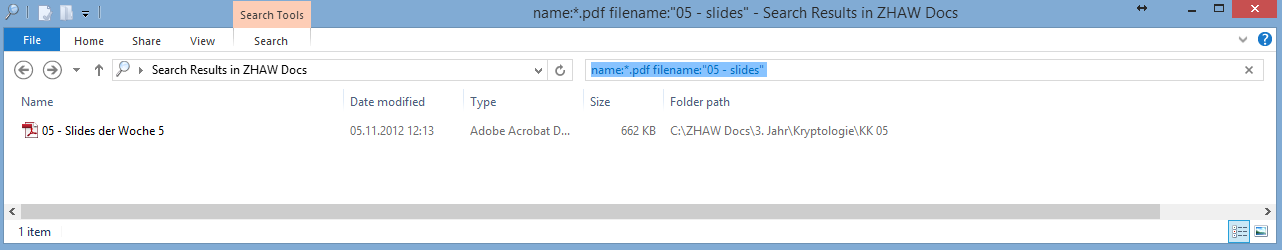
\includegraphics[width=1\textwidth]{Win8_Search2_extended_2.PNG} 
\caption[Erweiterte Suche 2 mit Windows 2]{Erweiterte Suche 2 mit Windows 2\\Quelle: eigener Screenshot}
\label{fig:Erweiterte Suche 2 mit Windows2}
\end{figure}

%==============  N E W  ==== S U B S E C T I O N ==============%
\subsection{Suche \#2 mit Lucene und Luke}

Bei der Suche mit Lucene findet Luke leider auch keinen Treffer.

\begin{figure}[h!]
\centering
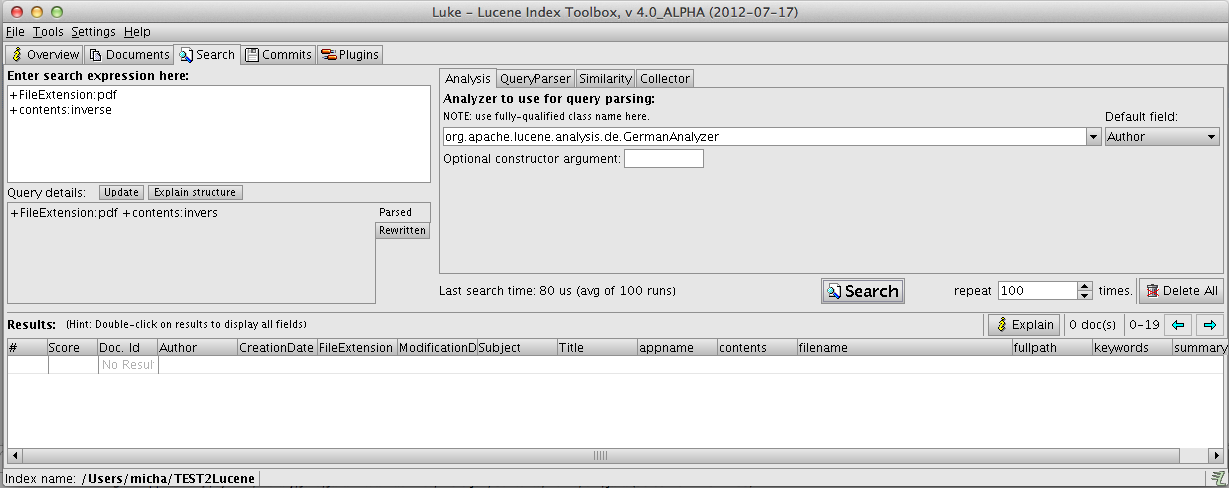
\includegraphics[width=1\textwidth]{Lucene_Search_2_1.PNG} 
\caption[Suche 2 mit Lucene]{Suche 2 mit Lucene\\Quelle: eigener Screenshot}
\label{fig:Suche 2 mit Lucene1}
\end{figure}

%==============  N E W  ==== S U B S E C T I O N ==============%
\subsection{Fazit zur Suche \#2}

Weder Windows noch Lucene konnten das gesuchte Dokument finden. Woran k�nnte dies liegen?\\
Beim Windows wurde bereits bei der Abbildung \ref{fig:Erweiterte Suche 2 mit Windows2} gezeigt, dass das Dokument grunds�tzlich gefunden wird. Jedoch indiziert Windows nicht den Inhalt des PDF.\\
Die Frage stellt sich nun, ob die Java Applikation Fehler enth�lt, so dass das PDF Dokument zwar indiziert wurde, jedoch nicht sein Inhalt.

\begin{figure}[h!]
\centering
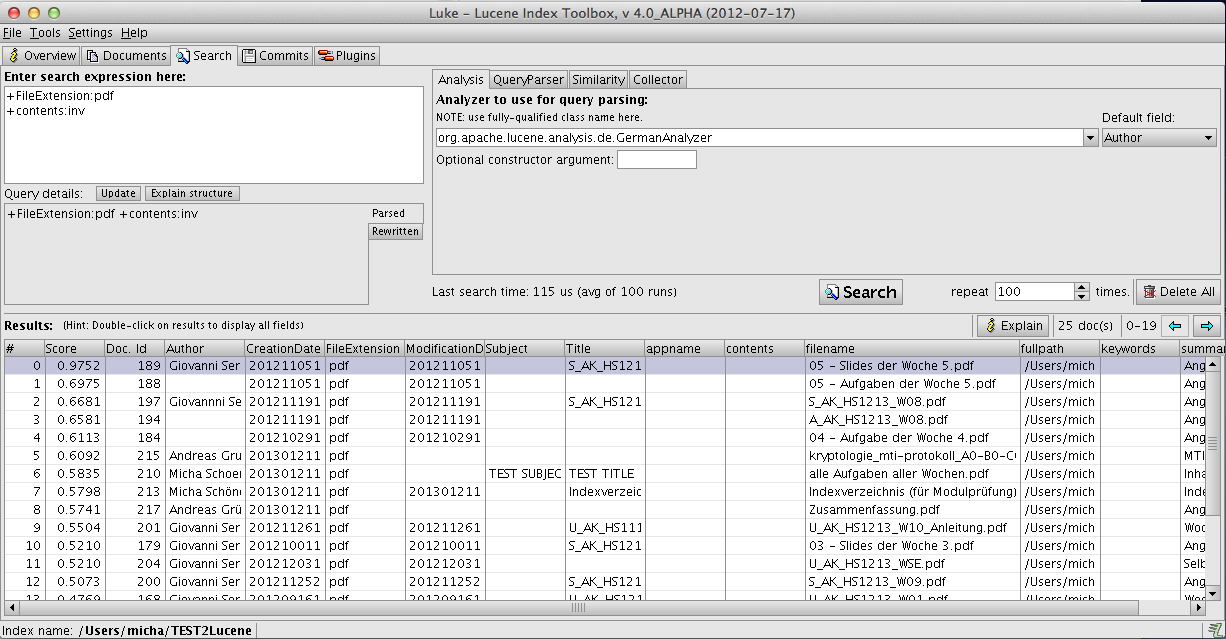
\includegraphics[width=1\textwidth]{Lucene_Search_2_2.PNG} 
\caption[Angepasste Suche 2 mit Lucene]{Angepasste Suche 2 mit Lucene\\Quelle: eigener Screenshot}
\label{fig:Suche 2 mit Lucene2}
\end{figure}

Abbildung \ref{fig:Suche 2 mit Lucene2} zeigt eindeutig, dass Lucene den Inhalt der PDF Files indiziert hat und das gesuchte File auch mit der besten Trefferrate findet.\\
Beim n�heren hinschauen ist ersichtlich, dass bei der Indizierung anstelle von \flqq inverse\frqq\ nur \flqq in\frqq\ eingelesen wurde. Auf die m�glichen Gr�nde wird hier nicht eingegangen.

Als Fazit der zweiten Suchanfrage kann man sagen, dass Lucene klar den Vorteil hat, dass PDF Inhalte indiziert werden und auch gefunden werden. Mit kleinen Anpassungen der Suchanfrage kann man das gesuchte Dokument ohne Probleme finden.








